\documentclass[compress]{beamer}%compress表示尽量压缩导航条
%\usetheme{Berlin}
\usepackage{thubeamer}
\usepackage{pgf}
\usepackage[UTF8,noindent]{ctex}%取消首行缩进

\usepackage{times} %设置文档中的所有英文为Times new roman字体
\usefonttheme{professionalfonts}    % 设置公式中的数学字体(wenzhong) http://bbs.ctex.org/forum.php?mod=viewthread&tid=76917

\setCJKsansfont[ItalicFont={KaiTi}]{SimSun}
%\logo{
\includegraphics[width=1.6cm,height=1.6cm]{logo.pdf}} %在每个页面的右下角插入logo
\usepackage{caption}
\setbeamertemplate{caption}[numbered]{}% Number float-like environments

%These 3 lines is used to correct the 'undefined control sequence \@@magyar@captionfix' error in TexLive2018
%Ref: https://tex.stackexchange.com/questions/426088/texlive-pretest-2018-beamer-and-subfig-collide
\makeatletter
\let\@@magyar@captionfix\relax
\makeatother
%

%bib reference
\usepackage[backend=bibtex,style=ieee,sorting=none]{biblatex}
\addbibresource{ref.bib}
\setbeamerfont{footnote}{size=\tiny}

\begin{document}

\graphicspath{{figures/}} % figures path
\captionsetup[figure]{font=footnotesize,labelfont=footnotesize}

\title{$ l_q $-规范最小化问题和压缩传感}
\author[王汉]{学生:王汉\\ \vskip 5pt 导师:王汉}
\institute[云南大学]{\small \vskip 38pt 云南大学}
\date{\small \vskip -22pt \today}
%\titlegraphic{
\includegraphics{logo.pdf}}
%\frame{
\begin{frame}
	\vspace{-10mm}
		\maketitle
	\vspace{-44mm}
	\begin{figure}[htbp]
		\begin{center}
			
\includegraphics[width=0.14\linewidth]{logo.pdf}
		\end{center}
	\end{figure}
\end{frame}
\section*{目录}
\begin{frame}
	\frametitle{\secname}
	\tableofcontents[sections={<1-5>}]
\end{frame}
  %\AtBeginSubsection[] {
  %\frame<handout:0> {
  %\frametitle{目录}
  %\tableofcontents[current,currentsubsection,sections={<1-5>}]
    %}
    %\addtocounter{framenumber}{-1}  %目录页不计算页码
  %}
  
\AtBeginSection[] {%在每一节前面加入目录显示当前节的目录结构
	\begin{frame}
		\frametitle{目录}
		\tableofcontents[currentsection,currentsubsection,hideothersubsections,sectionstyle=show/shaded,]
		\addtocounter{framenumber}{-1}  %目录页不计入页码
	\end{frame}
}




\section{背景问题定义}
\begin{frame}
	\frametitle{\secname~ }
	\begin{block}{CS基本问题}
		$x _ { 0 } \in R ^ { n }$是k稀疏的($\| x \| _ { 0}\leq k$),采样矩阵(测量矩阵)$A \in R ^ { m \times n }$,观测向量$y \in R ^ { m }$.
		$$y = A x _ { 0 }$$
	\end{block}
	\begin{block}{$l_0$-范数正则化问题}
$$\operatorname { min } _ { x } \frac { 1 } { 2 } \| y - A x \| _ { 2 } ^ { 2 } + \lambda \| x \| _ { 0 }$$
NP难问题。
\end{block}
\end{frame}
\begin{frame}

	\begin{block}{lasso问题}
$$\operatorname { min } _ { x } \frac { 1 } { 2 } \| y - A x \| _ { 2 } ^ { 2 } + \lambda \| x \| _ { 1 }$$
采用近端梯度下降法(PGD),IHT与ISTA。对压缩感知的非凸优化比L1范数凸优化方法的稀疏约束更强。\footfullcite{lyu2013comparison}压缩传感应用非凸模型会比凸模型跟为可取。\footfullcite{2010}
\end{block}
	\begin{block}{$l_q$问题($0<q\leq 1$)}
	$$\operatorname { min } _ { x } \frac { 1 } { 2 } \| y - A x \| _ { 2 } ^ { 2 } + \lambda \| x \| _ { q } ^ { q }$$
\end{block}	
\end{frame}
\section{研究方案}
\subsection{重定义问题}
\begin{frame}{重定义问题及解决方案}
  \begin{block}{近似原问题\footfullcite{9231911}}
$$\operatorname { min } _ { x } {F ( x )} = \frac { 1 } { 2 } \| y - A x \| _ { 2 } ^ { 2 } + \lambda \sum _ { i = 1 } ^ { n } \frac { | x _ { i } | } { ( | x _ { i } | + \varepsilon _ { i } ) ^ { 1 - q } }$$
  \end{block}
  \begin{block}{原问题}
$$\operatorname { lim } _ { \varepsilon _ { i } \rightarrow 0 ^ { + } } \frac { | x _ { i } | } { ( | x _ { i } | + \varepsilon _ { i } ) ^ { 1 - q } } = | x _ { i } | ^ { q }$$
  \end{block}
\end{frame}
\subsection{解决方案}
\begin{frame}{重定义问题及解决方案}
	\begin{block}{拓展重定义问题}
		${F ( x )}$拓展为$H ( x , c )$:
$$\operatorname { min } _ { x , c } H ( x , c ) = \frac { 1 } { 2 } \| y - A x \| _ { 2 } ^ { 2 } + \lambda \sum _ { i = 1 } ^ { n } \frac { | x _ { i } | } { ( | c _ { i } | + \varepsilon _ { i } ) ^ { 1 - q } } .$$
	\end{block}
	\begin{block}{两步问题}
		当$x=c$时,$H ( x , c )$退化为${F ( x )}$,可以表述为下列两步问题:
$$\left\{ \begin{array} { l } { \operatorname { min } _ { x } H ( x , \overline { c } ) = \frac { 1 } { 2 } \| y - A x \| _ { 2 } ^ { 2 } + \lambda \sum _ { i = 1 } ^ { n } \frac { | x _ { i } | } { ( | \overline { c } _ { i } | + \varepsilon _ { i } ) ^ { 1 - q } } } \\ { \operatorname { min } _ { c } | H ( \overline { x } , c ) - H ( \overline { x } , \overline { x } ) | } \end{array} \right.$$
	\end{block}
\end{frame}
\subsection{加权lasso问题及求解}
\begin{frame}{加权lasso问题}
	\begin{block}{加权lasso问题}
$$\operatorname { min } _ { x } \frac { 1 } { 2 } \| y - A x \| _ { 2 } ^ { 2 } + \lambda \sum _ { i = 1 } ^ { n } | w _ { i } x _ { i } |$$
\end{block}
	\begin{block}{求解方法}
		$$\left\{ \begin{array}{l}{ r ^ { t } = x ^ { t } + \beta A ^ { T } ( y - A x ^ { t } ) }\\{ x ^ { t + 1 } = \eta ( r ^ { t } ; \theta_t ) }\end{array} \right.$$
		其中$\theta _ { i } = \frac { \lambda } { ( | \overline { c } _ { i } | + \varepsilon _ { i } ) ^ { 1 - q } } ,$$\eta ( x ; \theta ) = \operatorname { sign } ( x ) \cdot \operatorname { max } \{ 0 , | x | - \theta \} .$
	\end{block}
\end{frame}
\section{论文提出算法}
\begin{frame}
\frametitle{\secname~ }
\begin{figure}[b]
	\centering
	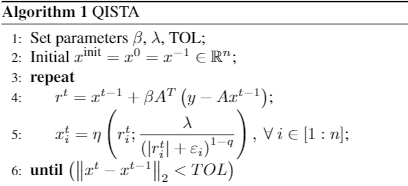
\includegraphics[width=0.5\textwidth]{4.png}
	\caption{QISTA伪代码}
\end{figure}

\end{frame}
\section{结果图}
\begin{frame}
	\frametitle{\secname~ }
\begin{figure}[b]
	\centering
	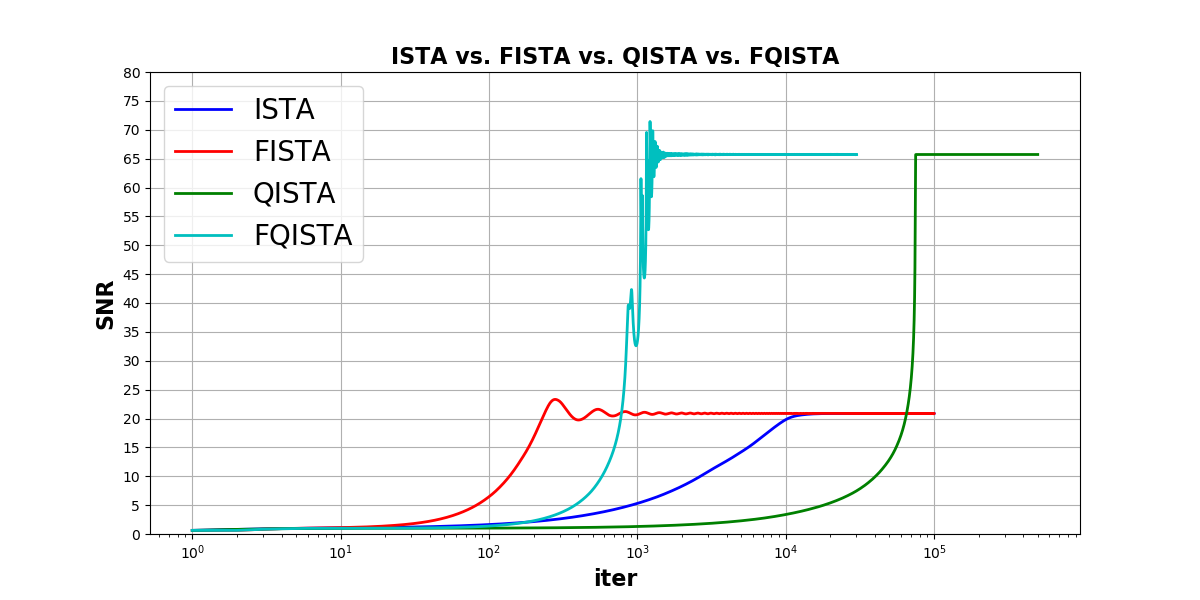
\includegraphics[width=0.4\textwidth]{n-m-k=1024-256-64-mean.png}
	\caption{n=1024,m=256,k=64}
\end{figure}
\begin{figure}[b]
	\centering
	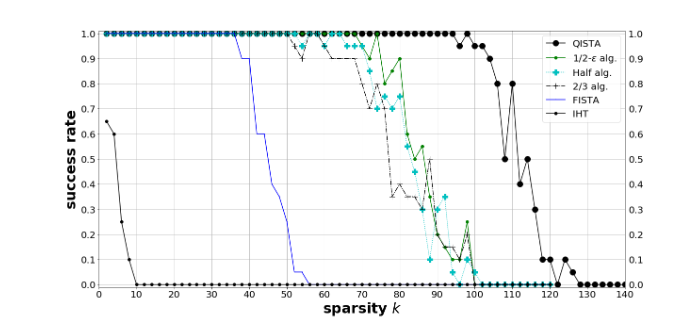
\includegraphics[width=0.4\textwidth]{5.png}
	\caption{QISTA,1/2算法,半阈值算法,2/3算法,FISTA和IHT的成功率随稀疏度的变化(n=1024,m=256)}
\end{figure}
\end{frame}
\section{Q\&A}
\begin{frame}{\secname~ }
	\begin{center}
 		\huge {\kaishu 结束,谢谢}
		
		\huge \textit {Q\&A}
	\end{center}
\end{frame}
\end{document}
